% arara: pdflatex: { synctex: yes }
% arara: makeindex: { style: ctuthesis }
% arara: bibtex

% The class takes all the key=value arguments that \ctusetup does,
% and a couple more: draft and oneside
\documentclass[twoside]{ctuthesis}

\ctusetup{
	preprint = \ctuverlog,
%	mainlanguage = english,
%	titlelanguage = czech,
	mainlanguage = czech,
	otherlanguages = {slovak,english},
	title-czech = {Firmware pro měřicí přístroj s mikrořadičem STM32G431},
	title-english = {Firmware for measuring instrument based on microcontroller STM32G431},
	%subtitle-czech = {Cesta do tajů kdovíčeho},
	%subtitle-english = {Journey to the who-knows-what wondeland},
	xdoctype = M,
	xfaculty = F3,
	department-czech = {Katedra měření},
	department-english = {Department of Measurement},
	author = {Bc. Petr David},
	supervisor = {doc. Ing. Jan Fischer, CSc.},
	%supervisor-specialist = {John Doe},
	%fieldofstudy-english = {Mathematical Engineering},
	%subfieldofstudy-english = {Mathematical Modelling},
	%fieldofstudy-czech = {Matematcké inženýrství},
	%subfieldofstudy-czech = {Matematické modelování},
	keywords-czech = {slovo, klíč},
	keywords-english = {word, key},
	day = 10,
	month = 5,
	year = 2023,
	specification-file = {DavidPetr-Zadani.pdf},
		front-specification = true,
	pkg-listings = true,
	%	front-list-of-figures = false,
	%	front-list-of-tables = false,
	%	monochrome = true,
	%	layout-short = true,
	}


\usepackage{gensymb}
\usepackage{calc}
\PassOptionsToPackage{hyphens}{url}
\usepackage{bm}
\usepackage{makecell}
\usepackage{amsmath}
\renewcommand\cellgape{\Gape[4pt]}
\setlength{\fboxsep}{0.02\linewidth}
\usepackage{diagbox}
\usepackage{epstopdf}
\usepackage{graphicx}
\usepackage{pdfpages}
\usepackage{caption}
\usepackage{svg}
\captionsetup[table]{name=Tab.}
\captionsetup[figure]{name=Obr.}

\newcommand{\sigline}[1]{\makebox[\widthof{#1~}]{.\dotfill}\\#1}
\numberwithin{table}{chapter}
\ctuprocess

\addto\ctucaptionsczech{%
	\def\supervisorname{Vedoucí}%
	\def\subfieldofstudyname{Studijní program}%
}




% Theorem declarations, this is the reasonable default, anybody can do what they wish.
% If you prefer theorems in italics rather than slanted, use \theoremstyle{plainit}
\theoremstyle{plain}
\newtheorem{theorem}{Theorem}[chapter]
\newtheorem{corollary}[theorem]{Corollary}
\newtheorem{lemma}[theorem]{Lemma}
\newtheorem{proposition}[theorem]{Proposition}

\theoremstyle{definition}
\newtheorem{definition}[theorem]{Definition}
\newtheorem{example}[theorem]{Example}
\newtheorem{conjecture}[theorem]{Conjecture}

\theoremstyle{note}
\newtheorem*{remark*}{Remark}
\newtheorem{remark}[theorem]{Remark}

\setlength{\parskip}{5ex plus 0.2ex minus 0.2ex}

% Abstract in Czech
\begin{abstract-czech}
Abstrakt v češtině
\end{abstract-czech}

% Abstract in English
\begin{abstract-english}
Abstract in English

\end{abstract-english}

% Acknowledgements / Podekovani
\begin{thanks}
Děkuji ČVUT, že mi je tak dobrou \emph{alma mater}.
\end{thanks}

% Declaration / Prohlaseni
\begin{declaration}
Prohlašuji, že jsem předloženou práci vypracoval samostatně, a že jsem uvedl veškerou použitou literaturu.

V Praze, \ctufield{day}.~\monthinlanguage{title}~\ctufield{year}
\end{declaration}


\begin{document}
\maketitle
\chapter{Úvod}

%!TEX ROOT=DavidPetrDP.tex
\chapter{Rozbor}





%!TEX ROOT=DavidPetrDP.tex
\chapter{Realizace FW}
\section{Struktura FW}
Jak vyplývá ze zadání, firmware vznikal v návaznosti na existujicí přístroj využívající stávající PC aplikací Zero eLab Viewer a jíž touto skutečností byl návrh firmware mikrokontroléru  částečně vymezen. V zájmu zpětné kompaktibility by totiž úpravy aplikace neměly ohrozit fungování předchozích implementací na jiných mikrokontrolérech, kterých je již celá řada. Především tedy  komunikační protokol, který i když je v některých případech limitující,  nemohl být upraven. Dále pak aplikace určuje, jaké softwarově definované přístoje lze implementovat a jaké budou mít možnosti ovládání či nastavení. Dále jsem se při návrhu zaměřil na tyto body

\begin{itemize}
	\item \textbf{Samostatná využitelnost jednotlivých přístrojových bloků}\\ 
	Rozdělit implementaci jednotlivých přístrojů do samostatně fungujících bloků je výhodné z 2 důvodů. Zaprvé lze tak jednodušeji výsledný FW přizpůsobit pro různé mikrokontroléry v závislosti na dostupných periferií a velikosti FLASH paměti.Druhým důvodem je pak možnost použití kódu i v jiných aplikacích.
	\item  \textbf{Jednoduchá záměna HW prostředků}\\
	Bylo žádoucí aby vznikající FW byl flexibilní co se týče použitých HW prostředků a tedy bylo jednoduché upravovat například použité piny, DMA kanály či čítače. Toto dále zjednodušuje další adaptaci firmware pro jiné MCU.	
	\item \textbf{Kompaktibilita s generátorem inicializačního kódu}\\	
	Nástroj STM32CubeMX velmi usnadňuje začátek vytváření FW díky využití grafického rozhraní pro definování počáteční konfigurace MCU. Pokud se zachová struktura generovaného kódu, lze pak nástroj opětovně využít v případě, že chceme jednoduše upravit HW konfiguraci.
\end{itemize}


\begin{figure}[H]
	\centering
	\includegraphics[width=0.9\linewidth]{Figs/Documentation/FW_Zavislosti}
	\caption{Kategorie zdrojového kodu a jejich posloupnost závislosti}
	\label{fig:fwzavislosti}
\end{figure}


\subsection{Využití možnosti přepínání mezi konfiguracemi}
Především z důvodů omezených hardwarových prostředků na různých mikrokontrolérech je využito možnosti přepínání různých přístrojových konfigurací. Konfigurací v tomto případě myslíme set nástrojů, které mohou být použity současně. Přístrojové moduly pak mohou sdílet periferie za předpokladu, že v dané konfiguraci je aktivní pouze jeden z těch modulů, který má přístup k dané periferii. Příkladem může být sdílení ADC převodníku modulem Voltmetru a modulem Osciloskopu, které pak tedy nemohou být aktivní zároveň. Jako je vidět na obrázku \ref{fig:zeroelab} hlavní okna PC aplikace.

\begin{figure}[H]
	\centering
	\includegraphics[width=0.7\linewidth]{Figs/Screenshots/ZeroElab}
	\caption{Hlavní okno aplikace Zero eLab Viewer zobrazující aktivní moduly dané konfigurace}
	\label{fig:zeroelab}
\end{figure}

\subsection{Využití LL ovladačů}
Jedná se o hardwarově orientovanou knihovnu dodávanou pro STM32 mikrokontrolery. Její využití je velmi podobné využití CMSIS ovladačů s tím rozdílem, že nabízí určité rozšířené možnosti portovatelnosti mezi jednotlivými rodinami mikrokontrolerů a sadu rozšiřujících API pro zjednodušení implementace některých úkonů jako je například inicializace periferií. K použití teto knihovny je oproti pravděpodobně známější knihovně HAL zapotřebí znalost jednotlivých periferií, jelikož velká část definovaných funkcí je pouze jednořádková modifikace registrů bez kontrol vstupních paramentrů a uživatel tedy musí být více obeznámen s tím co dělá. Výhodou oproti HAL je výrazně menší paměťová náročnost.\\

Pro vytvoření představy o rozdílnosti paměťové náročnosti jednotlivých knihoven jsem vytvořil pomocí STM32CubeMX dva minimální projekty, jejichž úkolem bylo nastavení systémových hodin blikání jednou LED. V prvním případě byly periferie RCC(Reset and clock control) a GPIO inicializovány prostřednictvím HAL knihovny a v druhém případě pomocí LL ovladačů a byly použity odpovídají zpožďovací funkce společně s přepínáním výstupu pinu. Výsledkem bylo, že  po zkompilování verze s HAL knihovnou využívala asi o 86 procent více FLASH.

\begin{table}[H]
	\begin{tabular}{l|ll}
		& FLASH   & RAM     \\ \hline
		LL ovlačače                       & 3.04 kB & 1,53 kB \\
		\multicolumn{1}{c|}{HAL ovladače} & 5,66 kB & 1,55 kB
	\end{tabular}
	\caption{Srovnání paměťové náročnosti jednoduchého programu s využitím různých knihoven}
	\label{tab:LL_HAL_MemoryUsage}
\end{table}	
\subsection{Core coupled memory CCM SRAM}


\section{Rozpoznání frekvence externího krystalu HSE}
Pro chod mikrokontroléru je zapotřebí zdroj hodinového signálu pro generování systémových hodin(System Core clock) dále jen SYSCLK. Jako základní varianta zdroje hodinového signálu se používá interní vysoko-rychlostní oscilátor(HSI), jehož výstupní frekvence ve srovnání s externími zdroji hodinového signálu vykazuje řádově vyšší nepřesnost a vyšší závislost na změnách teplot viz srovnávací tabulka \ref{tab:HSE}.Tento rozdíl je pak obzvlášť podstatný při realizaci funkce osciloskopu v režimu vzorkování v ekvivalentním čase(ETS), kde dochází k výraznému zkreslení měřeného signálu viz obrázek \ref{fig:signaldistortionhsi}. Na tomto obrázku je zobrazen zkreslený záznam signálu s G431 využívajícím HSI jako zdroj hodinového signálu a druhá stopa je měřena osciloskopem Rigol DS1052E jehož přesnost vzorkovací frekvence je $\pm0.005\%$ \cite{ScopeRigol}. Z obrázku je zřejmá vhodnost použití zdroje hodinového signálu s vyšší přesností než vykazuje HSI.

\begin{figure}[H]
	\centering
	\includegraphics[width=0.7\linewidth]{Figs/Graphs/SignalDistortion_HSI}
	\caption{Zkreslení průběhu měřeného signálu v důsledku nestability HSI převzato z \cite{DujavaDIP}}
	\label{fig:signaldistortionhsi}
\end{figure}

Jako zdroj vysokorychlostního externě získaného hodinové signálu(HSE) lze buď využít krystalu buzeného pomocí MCU(HSE crystal) nebo jiného externího zdroje signálu(HSE bypass). Případný externí signál musí pak splňovat nějaké podmínky a to například: pro STM32G431 musí být v rozsahu 4-48MHz a mít střídu 40-60\%. Ve výuce laboratorních měření na katedře měření jsou k dispozici krystaly různých výstupních frekvencí převážně pak 8 MHz, 12MHz a 16MHz.Pro  účely co nejflexibilnějšího laboratorního přístroje se zdálo účelné naprogramovat firmware pro použití s různými  oscilátory tohoto typu.Tedy aby funkce FW nebyla závislá na přítomnosti krystalu ani jeho výstupní frekvenci. Toho bylo docíleno změřením výstupní frekvence oscilátoru a nastavení výsledné frekvence systémových hodin pomocí interního obvodu fázového závěsu(PLL), tak aby výsledná frekvence SYSCLK nebyla na použitém krystalu závislá.


\begin{figure}[H]
	\centering
	\includegraphics[width=0.7\linewidth]{Figs/Diagrams/SVG/InputCapturePeriodMeasure.pdf}
	\caption{Zkreslení průběhu měřeného signálu v důsledku nestability HSI převzato z \cite{DujavaDIP}}
	\label{fig:signaldistortionhsi}
\end{figure}

Krátkodobá nestabilita frekvence (jitter)
\begin{table}[H]
	\begin{tabular}{l|rr}
		& $\Delta f$ f & $\Delta$ \\ \hline
		STM32G431 HSI 16 MHz     & $\pm$ 1\%       & $\pm$1\%      \\ \hline
		Adafruit krystal 16 MHz & $\pm$0.003\%   & $\pm$0.005\% 
	\end{tabular}
	\caption{}
	\label{tab:HSE}
\end{table}

\subsection{Měření frekvence HSE}
Existují různé způsoby měření frekvence externího hodinového signálu, ale jako nejúčelnější se v tomto případě zdálo použití čítače v režimu "Input capture"(IC) a měření délky periody externího signálu. Na rodině mikrokontrolérů STM32G4 mají čítače TIM16 a TIM17 možnost interně přivést HSE již se sníženou frekvencí. Frekvence HSE je totiž ještě před přivedením na vstup čítače zpracovaná obvodem, který frekvenci 32krát sníží. Pro tento vstup čítače se sníženou frekvencí se pak používá označení HSE32 jako je vidět na obrázku \ref{fig:tim16inputs} z dokumentace.

% TODO: \usepackage{graphicx} required
\begin{figure}[H]
	\centering
	\includegraphics[width=0.7\linewidth]{Figs/Documentation/TIM16_Inputs}
	\caption[Vstupy čítače TIM16]{Vstupy dostupné na kanálu číslo 1 čítače TIM16. Převzato z\cite{refG4}}
	\label{fig:tim16inputs}
\end{figure}

Měření periody signálu HSE32 probíhá potom tak, že měříme počet cyklů čítače mezi jednotlivými náběžnými hranami nebo sestupnými hranami. Tento počet cyklů nám pak určuje poměr mezi frekvencí externího hodinového signálu na vstupu $	f_{\text{IN}}$ a hodinového signálu, který pro svůj chod využívá periferie čítače $	f_{\text{TIM}}$. Pro správné měření je tedy podstatné, aby interní hodinový signál čítače byl výrazně vyšší než frekvence na měřeném vstupu. Pro získání přesnějšího odhadu vstupní frekvence můžeme zaznamenat více hodnot hodnot po sobě a ty  zprůměrovat. Frekvence vstupu je poté rovna:
\begin{equation}
	f_{\text{IN}}=\frac{f_{\text{TIM}}}{N_\text{p}}
\end{equation}
Pro určení frekvence HSE pak ještě musíme získanou hodnotu vynásobit 32:
\begin{equation}
	f_{\text{HSE}}=32 \cdot f_{\text{IN}}
\end{equation}
\subsection{Využití PLL}
Obvod PLL je další z možných zdrojů hodinového signálů systémových hodin, který má navíc programovatelné dělení a násobení vstupní frekvence. Jako vstup pak lze použít HSI nebo HSE ve stanovené rozsahu. Například 2.66-16MHz  pro stm32G431\cite{dataG431}. Dle obrázku \ref{fig:plldiagram} lze vidět, jak vstupní hodinový signál vstupujícího do PLL bloku  nejdříve prochází přes děličku signálu M, dále se hodinový signál násobí N a tento signál jde pak na 3 různé výstupy s vlastními děličkami. Dále v kapitole o ADC ukazuji výhodu této možnosti více výstupů z obvodu PLL, díky které vstupní hodiny ADC nemusí být závislé na frekvenci systémových hodin. 

\begin{figure}[H]
	\centering
	\includegraphics[width=0.6\linewidth]{Figs/Documentation/PLL_Diagram}
	\caption{Vyobrazení interního PLL bloku. Převzato z}
	\label{fig:plldiagram}
\end{figure}    

\subsection{Změna zdroje hodinového signálu systémových hodin}
Na obrázku \ref{fig:hsekonfigurace} je popsaný postup změny zdroje SYSCLK. Při změně vstupního signálu PLL nelze PLL používat, tedy je nejdříve zapotřebí přepnout systémové hodiny na interní oscilátor 16MHz. Dle doporučení v \cite{refG4} je při velkých rozdílech frekvencí mezi výstupem PLL(SYSCLK>80MHz) zapotřebí přidat mezikrok s využitím AHB předděličky hodinového signálu systémových hodin. hodnota předděličky se nastavuje RCC\_CFGR registru. Díky tomu například ve svém programu zmenším frekvenci systémových na polovinu tedy 78 MHz a pak až nastavuji jako zdroj HSI146. Doporučená doba setrvání v tomto mezikroku je alespoň $1\mu$s. V mém řešení program čeká 1ms s využitím připravených funkcí obsahujícím čekání v jednotkách ms.


\begin{figure}[H]
	\centering
	\includegraphics[width=1\linewidth]{Figs/Documentation/HSE_Konfigurace}
	\caption{Postup změny zdroje hodinového signálu}
	\label{fig:hsekonfigurace}
\end{figure}

\section{Realizace funkce Voltmetru}
\subsection{Nejistota měření}
\section{Realizace měření frekvence}
\subsection{Nejistota měření}
\section{Realizace funkce generátoru}
\subsection{Generování signálu}
\subsubsection{Využití CORDIC}    
CORDIC(COordinate ROtation DIgital Computer) je HW akcelerátor designovaný pro urychlení kalkulací vybraných matematický funkcí jako jsou trigonometrické a hyperbolické funkce.\cite{CORDIC}. Pro získání výsledku používá metody postupné aproximace. V m    případě trigonometrických funkcí algoritmus konverguje pro hodnoty $-\pi$ až $\pi$ radiánů. Algoritmus využívá číselné reprezentace s pevnou řádovou čárkou.  Výpočet funkce sinu daného úhlu pak probíhá postupnými rotacemi počátečního vektoru o postupně se zmenšující úhly dokud se výsledek dostatečně neblíž

\subsection{Generování šumu}
DAC převodník přítomný u MCU rodiny STM32G4 má implementován LFSR(linear feedback shift
register) umožňující pomocí převodníku generování pseudo-šumu o nastavitelném offsetu a amplitudě. Hodnota registru je vždy přepočítána po triggerování DAC převodníku podle specifického algoritmu popsaného na obrázku \ref{fig:noiselfsrcalculation}. Maskováním bitů tohoto registru dále můžeme nastavit offset a amplitudu výstupní signálu. Takto produkovaný šum má plochou spektrální distribuci a může být s určitou rezervou považován za bílý šum, s tím rozdílem, že narozdíl od pravého bílého šumu nemá Gaussovské(normální) rozdělení, ale rovnoměrné.
\begin{figure}
	\centering
	\includegraphics[width=0.7\linewidth]{Figs/Diagrams/NOISE_LFSR_Calculation}
	\caption{}
	\label{fig:noiselfsrcalculation}
\end{figure}

Jedním ze způsobu využití je ve spojitosti s průměrováním vzorků pro efektivní zvýšení rozlišení ADC převodníku. 
\begin{figure}
	\centering
	\includegraphics[width=0.7\linewidth]{Figs/Graphs/Noise}
	\caption{}
	\label{fig:noise}
\end{figure}

\section{Realizace osciloskopu}
Modul osciloskopu je nejkomplexnější z modulů implementovaných v této práci a též využívající nejvíce HW prostředků. K implementaci na STM32G431 jsem využil přítomnosti 2 ADC převodníku, triggerování pomocí analog watchdog (AWDG) funkce přítomných ADC převodníků, DMA řadiče a 2 vzájemně propojených zřetězených čítačů.
\subsection{Řešení triggerování osciloskopu}
Určení okamžiku náběžné nebo sestupné hrany vstupního signálu je podstatnou funkcí osciloskopu pro zobrazování jak přechodných jevů tak periodických průběhů signálu. Existuje více přístupů, jak takovou funkci implementovat. Jednou z nejjednoduších variant je SW orientované řešení, kdy  jsou naměřená data vždy cyklicky kontrolována, zda došlo k překročení zvolené napěťové úrovně a popřípadě zastavit další sběr dat. Takové řešení bylo například použito v původní variantě FW pro STM32F042 v práci \cite{BerlingerDIP}. Nevýhodou tohoto řešení je vyšší výpočetní náročnost ve srovnání s více HW zaměřenými řešeními, jaká jsou například využití komparátorů nebo funkce AWDG, kterou disponují ADC převodníky na mikrokontrolérech STM32G4 a kterou jsem se rozhodl uplatnit v této práci já.\\

AWDG umožňuje vyvolat přerušení v momentě, kdy se daném kanálu objeví napětí mimo nastavené rozmezí. Abychom mohli určit okamžik, kdy došlo k poklesu pod určitou úroveň(sestupná hrana) nebo naopak k překročení napěťové urovně(náběžná hrana) je potřeba využití AWDG ve dvou fázích znázorněných na obrázku \ref{fig:awdgtrigger}.

\begin{itemize}
	\item \textbf{Fáze 1}\\
	Při hledání okamžiku nástupní hrany v první fázi nejdříve nastavíme rozmezí nad střeženou napěťovou úrovní. Jakmile se napětí klesne mimo rozmezí dojde k přerušení a přesuneme se do fáze 2 
	\item \textbf{Fáze 2}\\
	V této fázi víme že signál je pod nastavenou napěťovou úrovní. Tedy nastavíme nové střežené rozmezí napětí a víme, že jakmile dojde k přerušení, že nastal okamžik, který chceme označit jako moment nástupní hrany a uložit si číslo vzorku, kdy k tomuto došlo.
\end{itemize}
\begin{figure}
	\centering
	\includegraphics[width=1\linewidth]{Figs/Graphs/AWDG_Trigger}
	\caption{2-fázové triggerování na nástupnou hranu signálu s využitím AWDG- převzato z \cite{DujavaDIP}}
	\label{fig:awdgtrigger}
\end{figure}

Po vyhodnocení, že došlo k události triggeru, potřebujeme zjistit číslo vzorku, kdy moment nastal a nastavit odměření zbývajících vzorků signálů, tak aby nové vzorky zapisované do kruhového bufferu nepřepsaly data vstupního signálu před touto událostí. Zde jsem využil dvou vzájemně propojených čítačů. Funkce prvního čítače je triggerování ADC převodníku a funkce druhého čítače je počítání odměřených vzorků a poté po triggeru zastavení triggerování po daném počtu vzorků. 

\begin{itemize}
	\item \textbf{Vzorkovací čítač }\\
	Vzorkovací čítač spouští vzorkování ADC převodníku. Ve spojitosti s osciloskopy se také používá termín generátor časové základny. V závislosti na propojení interních signálů daného mikrokontroléru můžeme pro spouštění signálu buď použít TRGO nebo jeden CC1 kanalů orkování může být buď Jako zdroj triggeru slouží UPDATE událost a kdy CNT registr dosáhne hodnoty ARR registru a čítač začíná počítat znovu od začátku. Hodnota prescaler a ARR registru tak určuje vzorkovací frekvenci. Vstupním hodinový signálem jsou interní hodiny o frekvenci systémových hodin. Navíc tento čítač operuje v slave modu "combine gated + reset", kdy tento čítač běží jen pokud na trigger vstupu(TRGI) je nastavena logická úroveň '1'. Jakmile dojde k poklesu na logickou úroveň(1) čítač se zastaví a zároveň se vyresetuje- tedy hodnota čítače CNT se vynuluje.
	
	\item \textbf{Čítač vzorků}\\
	Jak již název napovídá funkce tohoto čítače je určení pozice odebíraného vzorku v bufferu. Aktuální hodnota čítače odpovídá pozici v kruhovém bufferu následujícího snímaného vzorku. Tento čítač funguje ve funkci external clock 1 kdy čítač počítá náběžné hrany na vstupu TRGI. Na výstupu TRGO je potom stav čítače odpovídající enable bitu.
\end{itemize}

Vzájemné fungování by se pak dalo popsat následovně: pokud je zapnutý čítač vzorků, tak běží zároveň triggerovací čítač. Čítač vzorků čítá počet TRGO pulzů triggerovacího čítače a pokud čítač vzorkdů zastavíme, tak se zastaví triggerovací čítač a tím vzorkování ADC převodníkem. Pokud pak počítací čítač běží tzv 'one pulse' modu tak se oba čítače zastaví po odběru stanoveného počtu vzorků. 
\begin{figure}
	\centering
	\includegraphics[width=0.5\linewidth]{Figs/Diagrams/SamplingTimers_TRGI_TRGO}
	\caption{Vzájemné propojení dvou čítačů}
	\label{fig:samplingtimerstrgitrgo}
\end{figure}

\subsection{Módy vzorkování}
Pokud máme k dispozici pouze jeden ADC převodník, musíme v případě měření signálu na více kanálech vstup ADC převodníku přepínat mezi jednotlivými kanály. V případě využití dvou a více ADC převodníků máme daleko větší variablitu jak vzorkovat daný set analogových kanálů. Podrobněji se jednotlivým módům věnuje práce \cite{DujavaDIP}. STM32G431 má k dispozci 
2 ADC, které lze využít pro zvýšení vzorkovací frekvence, respektive zvýšení doby vzorkování pro stejnou vzorkovací frekvenci oproti použití 1 ADC. Výběr použitého módu vzorkování pak záleží na zvolených kanálech, respektive na jejich počtu a na jejich přítomnosti na jednotlivých ADC převodnících. Například kanál osciloskopu číslo 1 je na pinu PA0 a na tomto pinu také může být připojen na vstup převodníků ADC 1(kanál 1) a ADC 2(kanál1), ale například kanál osciloskopu číslo 3 je na pinu PA2, který se sice dá připojit na vstup převodníku ADC1, ale už se nedá připojit na vstup převodníku ADC2
\begin{table}[]
	\begin{tabular}{lccccc}
		Analogové kanály                & CH1         & CH2        & CH3     & CH4     & Vnitřní reference \\ \hline
		Přítomnost na Pinu               & PA0         & PA1        & PA2     & PA3     & -                 \\ \hline
		\multicolumn{1}{c}{Dostupné ADC} & ADC 1, ADC2 & ADC1, ADC2 & ADC1    & ADC1    & ADC1              \\ \hline
		Vnitřní kanál ADC                & Kanál 1     & Kanál 2    & Kanál 3 & Kanál 4 & Kanál 18         
	\end{tabular}
	\caption{Přehled jednotlivých analogových kanálů a jejich na dostupnosti na ADC převodnících}
	\label{tab:kanalyADC}
\end{table}

\subsubsection{Vzorkování 1 kanálu}
Pokud je zvolený kanál osciloskopu  přiveditelný na vstupy obou ADC převodníků, můžeme využít tzv. "Dual -interleaved modu". Tento režim spočívá ve střídavém vzorkování jedním převodníkem a v průběhu konverze odebraného vzorku vzorkováním převodníkem druhým. U mikrokontroléru rodiny STM32G4 minimální doba odběru jednoho vzorku(vzorkování + konverze) trvá 15 period hodinového signálu ADC převodníku. V případě dual - interleaved modu lze pak vzorkovat zvolený kanál druhým ADC v momentě kdy na prvním ADC převodníku ještě probíhá konverze viz obrázek \ref{fig:dualinterleaved}. Výsledně lze pak odebrat vzorek až každých 8 cyklů. Což dovoluje téměř zdvojnásobit maximální vzorkovací frekvenci. Druhou výhodou pak je možnost zvolení delší doby vzorkování při měření s nižší vzorkovací frekvencí více v kapitole \ref{Ch:SamplingTimeAndMaxInputRes}. \\

\begin{figure}[H]
	\centering
	\includegraphics[width=0.7\linewidth]{Figs/Screenshots/DualInterleaved}
	\caption{Převzato z \cite{refG4}}
	\label{fig:dualinterleaved}
\end{figure}

Problémem běžně popisovaného dual interleaved režimu je že vzorkování podřazeného ADC2 je spuštěno pevně stanový počet cyklů po vzorkování ADC1, což může zkreslit průběh měřeného signálu, pokud časový interval mezi odběry vzorků není stejná. V mé implementaci tedy používám něco jako Independent interleaved mod. V tomto režimu využívám output compare kanálu čítače,  abych spouštěl ADC převodníky střídavě tak, aby mezi po sobě jdoucími vzorky byla pokud možno stejná vzdálenost. Na výstupu čítače tedy je nastaven obdelníkový signál se střídou 50\% , ADC1 začíná vzorkovat na hranu náběžnou a ADC2 na hranu sestupnou. Každý cyklus čítače tedy  znamená odebrání 2 vzorků.\\

Oproti klasickému dual interleaved modu tento "independent interleaved mód" využívá nezávislého triggerování obou ADC převodníků. Nicméně stále je využito možnosti vyčítání naměřených dat ze sdílených data registů jako v případě obvyklého 'dual-interleaved' modu. Díky využití sdílených data registrů lze snížit vytížení DMA a AHB sběrnice a vyčítat data z obou ADC převodníků najednou a to s použitím 1 DMA kanálu přenášející 32 bitů . Přenos je pak spouštěn událostí dokončení konverze na ADC2.




\subsubsection{Vzorkování 2 a více kanálů}
Pokud je to možné  v případě zvolení 2 a více kanálů, je výhodné použít Dual Simultaneus režim, který nám umožní vzorkování více kanálů najednou. V mém FW jsem implementoval automatické přiřazování kanálů jednotlivým převodníků, podle jejich dostupnosti. Přiřazování probíhá tak že nejdříve se přiřadí kanály, které jsou dostupné pouze na jednom z převodníků a pak se posloupnosti kanálů doplní kanály dostupnými na obou převodnících tak, aby pokud možno oba ADC převodníky snímali stejný počet kanálů. Vznikají tak různé konfigurace na základě zvolených kanálů. Při analogových kanálech, tak jak jsou popsány v tabulce \ref{tab:kanalyADC} tak je při zvolení jakýkoliv 2 kanálů CH1-CH4 zajištěno snímání ve stejný čas, kromě kombinace CH3+Ch4, které jsou oba dostupné pouze na ADC1 a tedy musí být vzorkovány multiplexováním vstupu ADC převodníku. To má za následek v případě této kombinace sníženou maximální vzorkovací frekvenci v porovnání s jinými 2 kanálovými konfiguracemi. V případě zvolení 3 nebo 4 kanálů se pak ukázalo jako nejvhodnější řešení pevné nastavení skenování všech 4 kanálů, kdy jsou najednou snímany kanály CH1+CH3 a CH2+CH4. Po navzorkování bufferu je pak případně nezvolených kanál vyfiltrován z bufferu před posláním naměřených dat do počítače.
\begin{figure}[H]
	\centering
	\includegraphics[width=0.7\linewidth]{Figs/Screenshots/DualSimul2ADC}
	\caption{Dual Regular simultaneus mod převzato z \cite{refG4}}
	\label{fig:dualsimul2adc}
\end{figure}


\begin{figure}[H]
	\centering
	\includegraphics[width=0.7\linewidth]{Figs/Screenshots/DualSimul4Chn}
	\caption{Zpoždění kanálu 2 a 4 za kanálem 1 a 3 při použití Dual simultaneus modu a stroboskopickém vzorkování s ekvivalentní vzokovací frekvencí 78MHz}
	\label{fig:dualsimul4chn}
\end{figure}


\subsection{Nastavení délky vzorkování a vliv na maximální vstupní odpor}\label{Ch:SamplingTimeAndMaxInputRes}
Impedance analogového zdroje signálu, respektive sériový odpor($R_\text{AIN}$) mezi zdrojem a pinem ovlivňují proud nabíjející vzorkovací kondenzátor. Časová konstanta nabíjení $t_c$ potom určuje minimální dobu vzorkování, tak aby se vzorkovací kondenzátor měl čas nabít nabít na vstupní napětí(s tolerancí 1/2 LSB) $V_\text{AIN}$ jako je znázorněno na obrázku \ref{fig:samplingtimeandmaxinputresistance}. Čas vzorkování je limitován vzorkovací frekvencí a tedy pro různé vzorkovací frekvence existuje nějaký maximální vstupní odpor ($R_\text{AIN}$) takový, aby se měření neodchylovalo o více než $\pm0.5 \text{LSB}$.\\

\begin{figure}[H]
	\centering
	\includegraphics[width=0.9\linewidth]{Figs/Diagrams/SamplingTimeAndMaxInputResistance}
	\caption{ převzato z \cite{ADC_Acuraccy}}
	\label{fig:samplingtimeandmaxinputresistance}
\end{figure}

Doba vzorkování se nastavuje v počtu period hodinového signálu ADC (ADC\_CLK) převodníku s tím že na výběr je typicky pro daný ADC převodník sada dostupných hodnot s tím, že dále lze pak ovlivnit dobu vzorkování změnou frekvence již zmíněného ADC\_CLK. Jako nejlepší řešení se jevilo zvolit pro danou vzorkovací frekvenci a zvolený počet kanálů maximální možnou dobu vzorkování takovou, aby se stihly všechny zrovna zvolené kanály navzorkovat a zkonvertovat před tím, než přijde z triggerovacího čítače pokyn k dalšímu odběru vzorků. Mikrokontroler poté informuje uživatel skrz PC aplikaci o maximální impedanci zdroje signálu, aby měření nebylo zkresleno.

\begin{equation}
	t_c=(R_\text{ADC}+R_\text{AIN})\times C_\text{ADC}
\end{equation}

\begin{figure}[H]
	\centering
	\includegraphics[width=0.9\linewidth]{Figs/Graphs/WrongMaxRAIN}
	\caption{Efekt nedodržení maximálního vstupního odporu}
	\label{fig:wrongmaxrain}
\end{figure}


\section{Logický analyzátor}
\chapter{Ověření funkčnosti}







%\blindmathtrue

%\blinddocument

\chapter{Zhodnocení}
\chapter{Závěr}
\appendix

\printindex

\appendix

\bibliographystyle{acm}
\bibliography{ctutest}



\ctutemplate{specification.as.chapter}\end{document}